\chapter[Resultados Obtidos]{Resultados Obtidos}
Neste capítulo serão exibidos os resultados obtidos nesta primeira parte do projeto. Será falado dos resultados sobre o software de extração e da plataforma web.
\section{Software de Extração}
Na parte de extração dos dados foram criados dois codigos teste. O código \ref{code:handler} representa o uso da gem clockwork como um handler de frequência, o resultado obtido pelo uso do código pode ser visto na figura \ref{image:result_handler}. Já o código \ref{code:plugin} representa uma estrutura inicial de um plugin, nele é feito a conexão com o Elasticsearch, extraídos os dados de uma API, manipula esses dados e inserir no Elasticsearch.
\begin{lstlisting}[language={Ruby}, caption = {Código do Handler}, label = {code:handler}]
require 'clockwork'
require 'active_support/time'

# O modulo necessita ter o nome Clockwork
module Clockwork

	count_frequency = 0
	count_games = 0

	# Handler dos jobs
	handler do |job|
		if job.eql? 'frequency'
			count_frequency += 1
			print "A frequencia e: #{count_frequency}\n"
		elsif job.eql? 'games'
			count_games += 1
			print "O numero de jogos e: #{count_games}\n"
		end
	end

	# Define a frequencia dos jobs
	every(30.seconds, 'frequency')
	every(1.minutes, 'games')
end
\end{lstlisting}
\begin{figure}
\centering
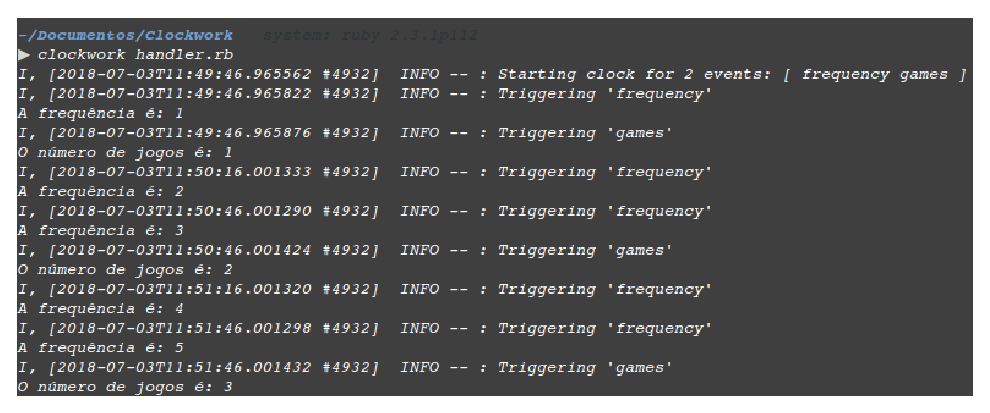
\includegraphics[scale=0.6]{figuras/result_handler.eps}
\caption{Resultado da Compilação do Handler}
\label{image:result_handler}
\end{figure}
\begin{lstlisting}[language={Ruby}, caption = {Código do Plugin}, label = {code:plugin}]
require 'httparty'
require 'elasticsearch'

# Classe que funciona como uma hash
class Game < Hash
	def put(key, value)
		self[key] = value;
	end
end

game = Game.new
# Conecta com o Elasticsearch
client = Elasticsearch::Client.new log: true
# Verifica se aquele index ja existe
if !client.indices.exists? index: 'test'
	client.indices.create index: 'test'
end
id = 730
url = 'http://store.steampowered.com/api/appdetails/?appids=' + id.to_s
# Extrai dados da API
response = HTTParty.get(url)
response.parsed_response
data = response["730"]["data"]
game.put("name", data["name"])
game.put("description", data["detailed_description"])
# Insere os dados no Elasticsearch
client.update index: 'test', type: 'game', id: 730, body: game.to_json
\end{lstlisting}
No decorrer do desenvolvimento da primeira parte do projeto, houve um mudança na política de privacidade da Steam, e isso modificou alguns dados que seriam extraídos, o principal foi o de número de donos. Antes de mudança a API do Steam Spy, providenciava um número quase exato do número de donos, após a mudança, agora a API providência apenas uma média estimada do número de donos. Isto alterar o projeto, já que agora não e possível mais fazer uma métrica exata da média de donos daquele gênero.